\documentclass[11pt]{article}
\usepackage{a4wide}
\usepackage{latexsym}
\usepackage{amssymb}
\usepackage{epic}
\usepackage{graphicx}
%\pagestyle{empty}
\newcommand{\tr}{\mbox{\sf true}}
\newcommand{\fa}{\mbox{\sf false}}
\newcommand{\bimp}{\leftrightarrow}


\begin{document}

\section*{
\begin{center}
Practical Assignment Part 1\\
Automated Reasoning 2IMF25\\
\end{center}
}

\begin{center}
Technische Universiteit Eindhoven\\
Jiahuan Zhang (j.4.zhang@student.tue.nl)\\
Hector Joao Rivera Verduzco (h.j.rivera.verduzco@student.tue.nl)\\

\end{center}
\date{\today}
\vspace{5mm}

\section*{Problem 1}

Six trucks have to deliver pallets of obscure building blocks to a magic factory. Every truck has a capacity of 7800 kg and can carry at most eight pallets. In total, the following has to be delivered:
\begin{itemize}
  \item Four pallets of nuzzles, each of weight 700 kg.
  \item A number of pallets of prittles, each of weight 800 kg.
  \item Eight pallets of skipples, each of weight 1000 kg.
  \item Ten pallets of crottles, each of weight 1500 kg.
  \item Five pallets of dupples, each of weight 100 kg.
\end{itemize}
Prittles and crottles are an explosive combination: they are not allowed to be put in the same truck.\\
Skipples need to be cooled; only two of the six trucks have facility for cooling skipples.\\
Dupples are very valuable; to distribute the risk of loss no two pallets of dupples may be in the same truck.\\
Investigate what is the maximum number of pallets of prittles that can be delivered, and show how for that number all pallets may be divided over the six trucks.

\vspace{4mm}

\subsection*{Solution:}

We generalize the problem to offer $m$ trucks to deliver the pallets. $m$ is a positive integer. Then we introduce some variables $t_{ij}$ for $i = 1, ..., m$ and $j = 1,...,5$, which represents the number of pallets of obscure building blocks $j$ on the $i$-th truck. $t_{ij}$ is a nature number. Every truck has a capacity, which is denoted as $C$, and the maximum number of pallets each truck can carry is $M$ kg.

The pallets of the same building blocks have the same weight, $weight(j)$. Each kind of building blocks has a predefined number, $\sharp pallets(j)$.

Now we consider the conditions for the delivery.

\begin{description}
  \item[Condition 1:] $t_{ij}$ should be no less than $0$.

  This is expressed by the formula
  \[ \bigwedge_{i,j:1 \leq i \leq m \wedge 1 \leq j \leq 5} t_{ij} \geq 0.\]
  \item[Condition 2:] Every truck has a capacity of $C$ kg.

  \[ \bigwedge_{i=1}^m  (\sum_{j=1}^5 t_{ij} \times weight(j)) \leq C .\]
  \item[Condition 3:] Every truck can carry at most eight pallets.

  \[ \bigwedge_{i=1}^m (\sum_{j=1}^5 t_{ij}) \leq M .\]
  \item[Condition 4:] The total numbers of the pallets of the other obscure building blocks should be exact the same as the given number.

  \[ \bigwedge_{1\leq j \leq 5} (\sum_{i=1}^m t_{ij}) = \sharp pallets(j) .\]

  \item[Condition 5:] Prittles and crottles are not allowed to be put in the same truck.

  \[ \bigwedge_{i=1}^m t_{i2}=0 \vee t_{i4}=0 .\]
  \item[Condition 6:] Only two of the trucks can deliver skipples.

      So let's assume the $m$-th and $m-2$-th trucks can deliver skipples.

  \[ t_{m3} + t_{(m-2)3} = M .\]
  \item[Condition 7:] No two pallets of dupples may be in the same truck.

  \[ \bigwedge_{i=1}^m t_{i5} \leq 1 .\]
\end{description}

The total formula now consists of the conjunction of all these
ingredients, that is,
\[ \bigwedge_{i,j:1 \leq i \leq m, 1 \leq j \leq 5} t_{ij} \geq 0 \;\; \wedge \]
\[ \bigwedge_{i=1}^m  (\sum_{j=1}^5 t_{ij} \times weight(j)) \leq C \;\; \wedge \]
\[ \bigwedge_{i=1}^m (\sum_{j=1}^5 t_{ij}) \leq M \;\; \wedge \]
\[ \bigwedge_{1\leq j \leq5, j\neq2} (\sum_{i=1}^m t_{ij}) = \sharp pallets(j) \;\; \wedge \]
\[ \bigwedge_{i=1}^m t_{i2}=0 \vee t_{i4}=0 \;\; \wedge \]
\[ t_{m3} + t_{(m-1)3} = M \;\; \wedge \]
\[ \bigwedge_{i=1}^m t_{i5} \leq 1 \]

This formula is easily expressed in SMT syntax. For Problem 1, we define $m = 6$, $M = 8$, $C = 7800$, and the table below.
\begin{center}
\begin{tabular}{|c|c|c|c|c|c|}
  \hline
  % after \\: \hline or \cline{col1-col2} \cline{col3-col4} ...
    & nuzzles & prittles & skipples & crottles & dupples \\
  $j$ & 1 & 2 & 3 & 4 & 5 \\
  $weight(j)$ & 700kg & 800kg & 1000kg & 1500kg & 100kg \\
  $\sharp pallets(j)$ & 4 & $n$ & 8 & 10 & 5 \\
  \hline
\end{tabular}
\end{center}

With the values above, we get the following Yices codes.

{\footnotesize

{\tt (benchmark Part1\_1.smt}

{\tt :logic $QF\_ALIA$}

{\tt :extrafuns (}

{\tt (t11 Int) (t12 Int) (t13 Int) (t14 Int) (t15 Int) }

{\tt (t21 Int) (t22 Int) (t23 Int) (t24 Int) (t25 Int) }

{\tt (t31 Int) (t32 Int) (t33 Int) (t34 Int) (t35 Int) }

{\tt (t41 Int) (t42 Int) (t43 Int) (t44 Int) (t45 Int) }

{\tt (t51 Int) (t52 Int) (t53 Int) (t54 Int) (t55 Int) }

{\tt (t61 Int) (t62 Int) (t63 Int) (t64 Int) (t65 Int) }

{\tt )}

{\tt :formula}

{\tt   (and}

{\tt (>= t11 0) (>= t12 0) (>= t13 0) (>= t14 0) (>= t15 0)}

{\tt (>= t21 0) (>= t22 0) (>= t23 0) (>= t24 0) (>= t25 0)}

$\cdots \cdots$

{\tt (>= t61 0) (>= t62 0) (>= t63 0) (>= t64 0) (>= t65 0) }

{\tt (<= (+ (* t11 700) (* t12 800) (* t13 1000) (* t14 1500) (* t15 100)) 7800)}

{\tt (<= (+ (* t21 700) (* t22 800) (* t23 1000) (* t24 1500) (* t25 100)) 7800)}

{\tt (<= (+ (* t31 700) (* t32 800) (* t33 1000) (* t34 1500) (* t35 100)) 7800)}

{\tt (<= (+ (* t41 700) (* t42 800) (* t43 1000) (* t44 1500) (* t45 100)) 7800)}

{\tt (<= (+ (* t51 700) (* t52 800) (* t53 1000) (* t54 1500) (* t55 100)) 7800)}

{\tt (<= (+ (* t61 700) (* t62 800) (* t63 1000) (* t64 1500) (* t65 100)) 7800) }

{\tt (<= (+ t11 t12 t13 t14 t15) 8)}

{\tt (<= (+ t21 t22 t23 t24 t25) 8)}

{\tt (<= (+ t31 t32 t33 t34 t35) 8)}

{\tt (<= (+ t41 t42 t43 t44 t45) 8)}

{\tt (<= (+ t51 t52 t53 t54 t55) 8)}

{\tt (<= (+ t61 t62 t63 t64 t65) 8)}

{\tt (= (+ t11 t21 t31 t41 t51 t61) 4)}

{\tt (= (+ t12 t22 t32 t42 t52 t62) 18)}

{\tt (= (+ t13 t23 t33 t43 t53 t63) 8)}

{\tt (= (+ t14 t24 t34 t44 t54 t64) 10)}

{\tt (= (+ t15 t25 t35 t45 t55 t65) 5)}

{\tt (or (= t12 0) (= t14 0)) }

{\tt (or (= t22 0) (= t24 0)) }

{\tt (or (= t32 0) (= t34 0)) }

{\tt (or (= t42 0) (= t44 0)) }

{\tt (or (= t52 0) (= t54 0)) }

{\tt (or (= t62 0) (= t64 0)) }

{\tt (or}

{\tt (= (+ t43 t63) 8) }

{\tt (<= t15 1) (<= t25 1) (<= t35 1) (<= t45 1) (<= t55 1) (<= t65 1)}

{\tt )) }
}

Applying {\tt yices-smt -m Part1\_1.smt} several times, we find when the number of pallets of prittles is 19, it is UNSAT. When the number is 18, it is SAT. Therefore, we conclude that the maximal number of pallets of prittles is 18.
The following result is yielded within a fraction of a second:

{\footnotesize

{\tt sat}

{\tt (= t52 7)}

{\tt (= t11 0)}

{\tt (= t14 5)}

{\tt (= t34 0)}

{\tt (= t21 4)}

{\tt (= t15 1)}

{\tt (= t44 2)}

{\tt (= t45 1)}

{\tt (= t54 0)}

{\tt (= t33 0)}

{\tt (= t35 0)}

{\tt (= t51 0)}

{\tt (= t23 0)}

{\tt (= t53 0)}

{\tt (= t65 1)}

{\tt (= t13 0)}

{\tt (= t62 0)}

{\tt (= t25 1)}

{\tt (= t32 8)}

{\tt (= t41 0)}

{\tt (= t63 4)}

{\tt (= t43 4)}

{\tt (= t42 0)}

{\tt (= t12 0)}

{\tt (= t64 0)}

{\tt (= t55 1)}

{\tt (= t22 0)}

{\tt (= t24 3)}

{\tt (= t61 0)}

{\tt (= t31 0)}

}

\begin{table}
  \centering
  \begin{tabular}{|l|c|c|c|c|c|}
    \hline
    % after \\: \hline or \cline{col1-col2} \cline{col3-col4} ...
     & nuzzles & prittles & skipples & crottles & dupples \\
    Truck 1 & 0 & 0 & 0 & 5 & 1 \\
    Truck 2 & 4 & 0 & 0 & 3 & 1 \\
    Truck 3 & 0 & 8 & 0 & 0 & 0 \\
    Truck 4 & 0 & 0 & 4 & 2 & 1 \\
    Truck 5 & 0 & 7 & 0 & 0 & 1 \\
    Truck 6 & 0 & 3 & 4 & 0 & 1 \\
    \hline
  \end{tabular}
\end{table}

\subsection*{Remark}
In this problem, we are required to find out the maximum number of the pallets of prittles. Such kind of maximum values searching is likely to become very time-consuming since there is no explicitly close upper bound to start the searching.

For this problem, we first find out the theoretically possible maximum number of the pallets of prittles through calculation. Because the capacity of each track is given, and it is also provided the total weights of the pallets of the other obscure building blocks, we can estimate the number.

  $\frac{7800 \times 6 - 700\times4 - 1000\times8 - 1500\times10 - 100\times5}{800} = 25.625$

Because the number of pallets is a nature number, the maximum number should not be more than 25. Therefore, we can start the debugging from $n = 25$ downwards.

\subsection*{Generalization}

We generalized all the invariants except the total number of kinds of the building blocks in this problem, because most of the requirements come from the features of different building blocks, which indicates that adding more different building blocks will generate more requirements, and as a consequent, the entire formula we summarized in the end of the solution is not applicable.

One more note is for the people who are interested in setting the number of trucks, $m$, larger than $10$. They need to care care about the notations of the variables $t_{ij}$. For instance, the number of pallets of building blocks labeled $1$ on the eleventh truck, $t_{11,1}$, is expressed as  $t111$ in Yices codes. This expression can also represent the number of pallets of building blocks labeled $11$ on the first truck, $t_{1,11}$. An extra symbol between the two numbers $i$ and $j$ is required to avoid this ambiguity.

Decreasing the number of trucks is more of interest. We did some testing to figure out how many pallets of prittles can satisfy these conditions with fewer trucks. When there are five trucks in all, ten pallets of prittles can be delivered with the satisfiability of the conditions. With fewer trucks, no satisfiability is reached. Since one truck can only deliver one pallet of drupples due to the condition, the number of trucks has to be larger than the number of pallets of drupples for delivery. It can be expressed as this
\[ \sum_{i=1}^m t_{i5}\leq m \]


\section*{Problem 2}

Give a chip design containing three power components and eight regular components satisfying the following constraints:
\begin{itemize}
  \item The width of the chip is 29 and the height is 22.
  \item All power components have width 4 and height 2.
  \item The sizes of the eight regular components are $9 \times 7$, $12 \times 6$, $10 \times 7$, $18 \times 5$, $20 \times 4$, $10 \times 6$, $8 \times 6$ and $10 \times 8$, respectively.
  \item All components may be turned 90, but may not overlap.
  \item In order to get power, all regular components should directly be connected to a power component, that is, an edge of the component should have at least one point in common with an edge of the power component.
  \item Due to limits on heat production the power components should be not too close: their centres should differ at least 17 in either the $x$ direction or the $y$ direction (or both).
\end{itemize}

\vspace{4mm}

\subsection*{Solution:}
First of all, we assume the chip plan is a positive plane whose left-bottom corner has coordinate $(0, 0)$, and right-top corner has coordinate $(29, 22)$.
Next, we introduce coordinates to each corner of each components $(x_{ij}, y_{ij})$ to specify them.
See below.

\begin{enumerate}
  \item For the three power components:\\
  Power component 1 has coordinates $(x_{11}, y_{11})$, $(x_{12}, y_{11})$, $(x_{12}, y_{11})$ and $(x_{12}, y_{12})$.\\
  Power component 2 has coordinates $(x_{21}, y_{21})$, $(x_{22}, y_{21})$, $(x_{22}, y_{21})$ and $(x_{22}, y_{22})$.\\
  Power component 3 has coordinates $(x_{31}, y_{31})$, $(x_{32}, y_{31})$, $(x_{32}, y_{31})$ and $(x_{32}, y_{32})$.
  \item For the eight regular components:\\
  Regular component 1 has coordinates $(n_{11}, m_{11})$, $(n_{12}, m_{11})$, $(n_{12}, m_{11})$ and $(n_{12}, m_{12})$.\\
  Regular component 2 has coordinates $(n_{21}, m_{21})$, $(n_{22}, m_{21})$, $(n_{22}, m_{21})$ and $(n_{22}, m_{22})$.

  $\cdots \cdots$

  Regular component 8 has coordinates $(n_{81}, m_{81})$, $(n_{82}, m_{81})$, $(n_{82}, m_{81})$ and $(n_{82}, m_{82})$.
\end{enumerate}
Thus, we plan to put the components onto the plan in terms of the constraints.

\begin{description}
  \item[Constraint 1:] Now the chip is a positive plane, so all the coordinates should be positive. The width of the chip is 29 and the height is 22.

  Then we have
  \[  \bigwedge_{i=1}^3 29 \geq x_{i2} \geq x_{i1} \geq 0 \wedge 22 \geq y_{i2} \geq y_{i1} \geq 0 \;\; \wedge \]
  \[  \bigwedge_{i=1}^8 29 \geq n_{i2} \geq n_{i1} \geq 0 \wedge 22 \geq m_{i2} \geq m_{i1} \geq 0 \]
  \item[Constraint 2:] All power components have width 4 and height 2,
  and the sizes of the eight regular components are $9 \times 7$, $12 \times 6$, $10 \times 7$, $18 \times 5$, $20 \times 4$, $10 \times 6$, $8 \times 6$ and $10 \times 8$, respectively.
  All components may be turned 90.

  Then we have
  \[  \bigwedge_{i=1}^3 ((x_{i2} - x_{i1} = 4 \; \wedge \; y_{i2} - y_{i1} = 2) \;\; \vee \]
  \[ (x_{i2} - x_{i1} = 2 \; \wedge \; y_{i2} - y_{i1} = 4)) \]
  So do the coordinates for the Regular components. However their sizes are distinct,
  this makes more writing and coding. Here we only show the clause for the first regular component,
  whose size is $9 \times 7$. \\
  \[ (n_{12} - n_{11} = 9 \; \wedge \; m_{12} - m_{11} = 7) \;\; \vee (n_{12} - n_{11} = 7 \; \wedge \; m_{12} - m_{11} = 9) \]
  \item[Constraint 3:] All components may not overlap.

\begin{center}
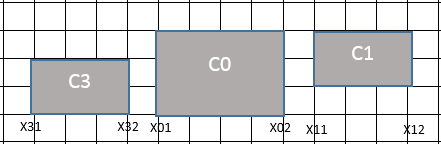
\includegraphics[width=0.5\textwidth]{Part1_2_1.png}
\end{center}
  As the figure shows, only if a component's $x_{i1}$ is larger than the other one's $x_{k2}$, then these two components are not overlapped. We also have the case in the y direction.

  Among the power components:

  \[  \bigwedge_{i,k: 1 \leq i \leq 3, 1 \leq k \leq 3, i \neq k}
  x_{i2} \leq x_{k1} \; \vee \; x_{k2} \leq x_{i1} \; \vee \; y_{i2} \leq y_{k1} \; \vee \; y_{k2} \leq y_{i1} \]

  Among the regular components:

  \[  \bigwedge_{i,k: 1 \leq i \leq 8, 1 \leq k \leq 8, i \neq k}
  n_{i2} \leq n_{k1} \; \vee \; n_{k2} \leq n_{i1} \; \vee \; m_{i2} \leq m_{k1} \; \vee \; m_{k2} \leq m_{i1}  \]

  Between the power components and the regular components:

  \[  \bigwedge_{i,k: 1 \leq i \leq 3, 1 \leq k \leq 8, i \neq k}
   x_{i2} \leq n_{k1} \; \vee \; n_{k2} \leq x_{i1} \; \vee \; y_{i2} \leq m_{k1} \; \vee \; m_{k2} \leq y_{i1} \]

  \item[Constraint 4:] An edge of the regular component should have at least one point in common with an edge of the power component.

\begin{center}
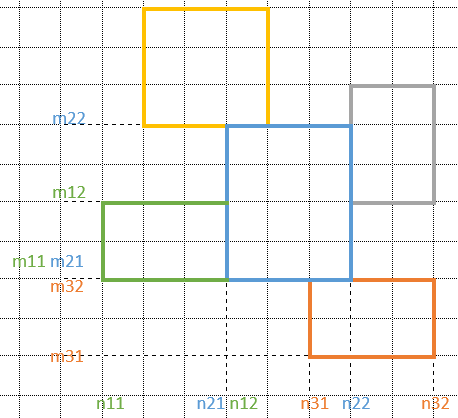
\includegraphics[width=0.5\textwidth]{Part1_2_2.png}
\end{center}

  As the figure above shows, if two components are touched at least one point, then at least one coordinate of a component is the same as the other one. We consider it from the inverse way to make the clauses simpler. If two components have the same $x_{i1}$ value, only if their $y$-direction sides are not touched, then these two components are not in common with an edge of each other.
  We denote this condition as follows.

  \[  \bigwedge_{i,k: 1 \leq i \leq 3, 1 \leq k \leq 8}
  ((x_{i2} = n_{k1} \; \vee \; x_{i1} = n_{k2}) \; \wedge \;
  \neg (y_{i2} < m_{k1} \vee m_{k2} < y_{i1}) \; \vee \; \]
  \[  ((y_{i2} = m_{k1} \; \vee \; y_{i1} = m_{k2}) \; \wedge \;
  \neg (x_{i2} < n_{k1} \vee n_{k2} < x_{i1}))) \]
  \item[Constraint 5:] The power components' centres should differ at least 17 in either the $x$ direction or the $y$ direction (or both).

  The centers of the power components are $(x_{i1} + \frac{x_{i2} - x_{i1}}{2}, y_{i1} + \frac{y_{i2} - y_{i1}}{2} )$.

  For each pair of the power components, we have

  \[  \bigwedge_{i,k: 1 \leq i < k \leq 3}
  [ (x_{i1} + \frac{x_{i2} - x_{i1}}{2}) - (x_{k1} + \frac{x_{k2} - x_{k1}}{2}) \geq 17 \; \vee \; \]
  \[ (x_{k1} + \frac{x_{k2} - x_{k1}}{2}) - (x_{i1} + \frac{x_{i2} - x_{i1}}{2}) \geq 17 \; \vee \; \]
  \[ (y_{k1} + \frac{y_{k2} - y_{k1}}{2}) - (y_{i1} + \frac{y_{i2} - y_{i1}}{2}) \geq 17 \; \vee \; \]
  \[ (y_{i1} + \frac{y_{i2} - y_{i1}}{2}) - (y_{k1} + \frac{y_{k2} - y_{k1}}{2}) \geq 17 ] \]


\end{description}

Making a conjunction of all the clauses derived from the constraints, we made the Yices smt cods.

This formula is easily expressed in SMT syntax.

{\footnotesize

{\tt (benchmark Part1\_2.smt}

{\tt :logic $QF\_LIA$}

{\tt :extrafuns (}

{\tt (x11 Int) (x12 Int) (y11 Int) (y12 Int)}

{\tt (x21 Int) (x22 Int) (y21 Int) (y22 Int)}

{\tt (x31 Int) (x32 Int) (y31 Int) (y32 Int)}

{\tt (n11 Int) (n12 Int) (m11 Int) (m12 Int)}

{\tt (n21 Int) (n22 Int) (m21 Int) (m22 Int)}

$\cdots \cdots$

{\tt (n81 Int) (n82 Int) (m81 Int) (m82 Int)}

{\tt )}

{\tt :formula (and}

{\tt (>= 29 x12) (>= x12 x11) (>= x11 0) (>= 22 y12) (>= y12 y11) (>= y11 0)}

{\tt (>= 29 x22) (>= x22 x21) (>= x21 0) (>= 22 y22) (>= y22 y21) (>= y21 0)}

{\tt (>= 29 x32) (>= x32 x31) (>= x31 0) (>= 22 y32) (>= y32 y31) (>= y31 0)}

{\tt (>= 29 n12) (>= n12 n11) (>= n11 0) (>= 22 m12) (>= m12 m11) (>= m11 0)}

{\tt (>= 29 n22) (>= n22 n21) (>= n21 0) (>= 22 m22) (>= m22 m21) (>= m21 0)}

$\cdots \cdots$

{\tt (>= 29 n82) (>= n82 n81) (>= n81 0) (>= 22 m82) (>= m82 m81) (>= m81 0)}

{\tt (or (and (>= 29 x12) (>= 22 y12) (= (- x12 x11) 4) (= (- y12 y11) 2))}

{\tt (and (>= 22 x12) (>= 29 y12) (= (- y12 y11) 4) (= (- x12 x11) 2)))}

$\cdots \cdots$

{\tt (or (and (= (- x32 x31) 4) (= (- y32 y31) 2)) (and (= (- x32 x31) 2) (= (- y32 y31) 4)))}

{\tt (or (and (= (- n12 n11) 9) (= (- m12 m11) 7)) (and (= (- n12 n11) 7) (= (- m12 m11) 9)))}

$\cdots \cdots$

{\tt (or (and (= (- n82 n81) 10) (= (- m82 m81) 8)) (and (= (- n82 n81) 8) (= (- m82 m81) 10)))}

{\tt ;; not overlap among power components}

{\tt (or (<= x12 x21) (<= x22 x11) (<= y12 y21) (<= y22 y11))}

{\tt (or (<= x12 x31) (<= x32 x11) (<= y12 y31) (<= y32 y11))}

{\tt (or (<= x32 x21) (<= x22 x31) (<= y32 y21) (<= y22 y31))}

{\tt ;; not overlap among regular components}

{\tt (or (<= n12 n21) (<= n22 n11) (<= m12 m21) (<= m22 m11))}

{\tt (or (<= n12 n31) (<= n32 n11) (<= m12 m31) (<= m32 m11))}

$\cdots \cdots$

{\tt (or (<= n72 n81) (<= n82 n71) (<= m72 m81) (<= m82 m71))}

{\tt ;;not overlap between power components and regular ones}

{\tt (or (<= x12 n11) (<= n12 x11) (<= y12 m11) (<= m12 y11))}

{\tt (or (<= x12 n21) (<= n22 x11) (<= y12 m21) (<= m22 y11))}

$\cdots \cdots$

{\tt (or (<= x32 n81) (<= n82 x31) (<= y32 m81) (<= m82 y31))}

{\tt ;;Constraint 4}

{\tt (or}

{\tt (and (or (= x11 n12) (= x12 n11)) (not (or (< y12 m11) (> y11 m12))))}

{\tt (and (or (= x21 n12) (= x22 n11)) (not (or (< y22 m11) (> y21 m12))))}

$\cdots \cdots$

{\tt (and (or (= y31 m12) (= y32 m11)) (not (or (< x32 n11) (> x31 n12))))}

{\tt )}

$\cdots \cdots$

{\tt (or}

{\tt (and (or (= x11 n82) (= x12 n81)) (not (or (< y12 m81) (> y11 m82))))}

{\tt (and (or (= x21 n82) (= x22 n81)) (not (or (< y22 m81) (> y21 m82))))}

$\cdots \cdots$

{\tt (and (or (= y31 m82) (= y32 m81)) (not (or (< x32 n81) (> x31 n82))))}

{\tt )}

{\tt ;;Constraint 5}

{\tt (or (>= (- (+ x11 (/ (- x12 x11) 2)) (+ x21 (/ (- x22 x21) 2))) 17)}

{\tt (>= (- (+ x21 (/ (- x22 x21) 2)) (+ x11 (/ (- x12 x11) 2))) 17)}

{\tt (>= (- (+ y11 (/ (- y12 y11) 2)) (+ y21 (/ (- y22 y21) 2))) 17)}

{\tt (>= (- (+ y21 (/ (- y22 y21) 2)) (+ y11 (/ (- y12 y11) 2))) 17))}

$\cdots \cdots$

{\tt (or (>= (- (+ x11 (/ (- x12 x11) 2)) (+ x31 (/ (- x32 x31) 2))) 17)}

{\tt (>= (- (+ x31 (/ (- x32 x31) 2)) (+ x11 (/ (- x12 x11) 2))) 17)}

{\tt (>= (- (+ y11 (/ (- y12 y11) 2)) (+ y31 (/ (- y32 y31) 2))) 17)}

{\tt (>= (- (+ y31 (/ (- y32 y31) 2)) (+ y11 (/ (- y12 y11) 2))) 17))}

{\tt ))}
}

Applying {\tt yices-smt -m part$1\_2$.smt}, we test out a satisfiable chip design plan.

{\footnotesize

{\tt sat}

{\tt(= x11 4)}

{\tt(= x12 6)}

{\tt(= y11 2)}

{\tt(= y12 6)}

{\tt(= x21 0)}

{\tt(= x22 4)}

{\tt(= y21 20)}

{\tt(= y22 22)}

{\tt(= x31 21)}

{\tt(= x32 23)}

{\tt(= y31 10)}

{\tt(= y32 14)}

{\tt(= n11 12)}

{\tt(= n12 21)}

{\tt(= m11 10)}

{\tt(= m12 17)}

{\tt(= n21 23)}

{\tt(= n22 29)}

{\tt(= m21 10)}

{\tt(= m22 22)}

{\tt(= n31 4)}

{\tt(= n32 22)}

{\tt(= m31 17)}

{\tt(= m32 22)}

{\tt(= n41 14)}

{\tt(= n42 21)}

{\tt(= m41 0)}

{\tt(= m42 10)}

{\tt(= n51 0)}

{\tt(= n52 4)}

{\tt(= m51 0)}

{\tt(= m52 20)}

{\tt(= n61 5)}

{\tt(= n62 11)}

{\tt(= m61 6)}

{\tt(= m62 16)}

{\tt(= n71 6)}

{\tt(= n72 14)}

{\tt(= m71 0)}

{\tt(= m72 6)}

{\tt(= n81 21)}

{\tt(= n82 29)}

{\tt(= m81 0)}

{\tt(= m82 10)}

}

\begin{center}
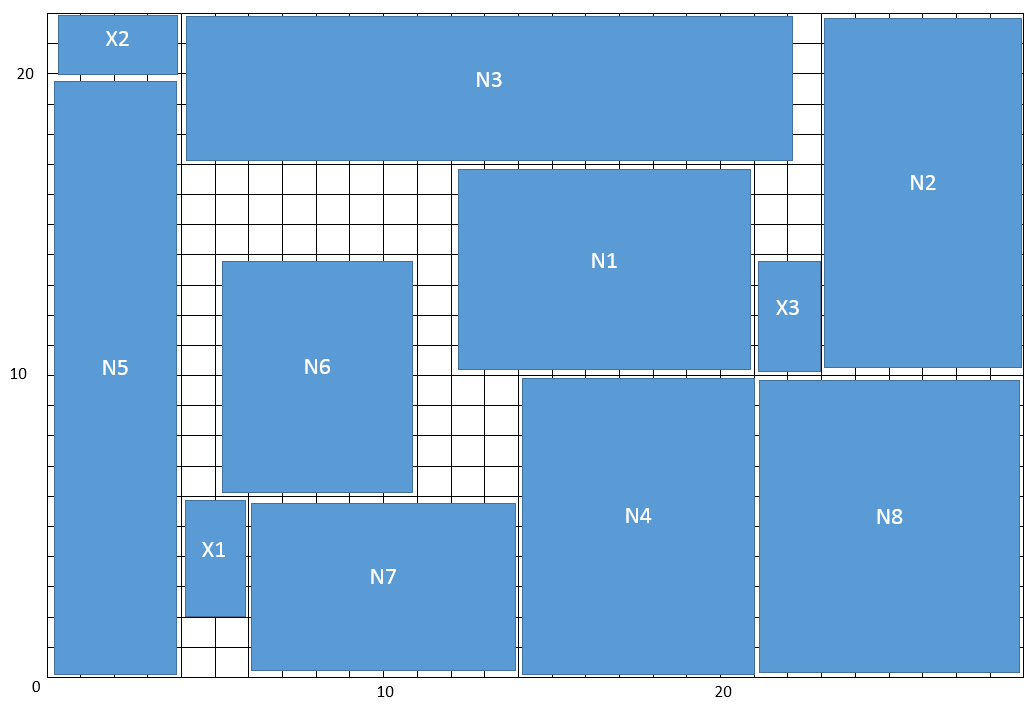
\includegraphics[width=0.8\textwidth]{Part1_2_3.png}
\end{center}

\subsection*{Remark:}

\subsection*{Generalization:}

\section*{Problem 3}

The goal of this problem is to exploit the power of the recommended tools rather than elaborating the questions by hand

\begin{description}
  \item[(a)] In mathematics, a \emph{group} is defined to be a set $G$ with an element $I \epsilon G$, a binary operator $\ast$ and a unary operator \emph{inv} satisfying
      \begin{center}
      $ x \ast(y \ast z)=(x\ast y) \ast z, x \ast I = x $ and $ x \ast inv(x) = I, $
      \end{center}
      for all $x, y, z \epsilon G$. Determine whether in every group each of the four properties
      \begin{center}
      $I \ast x = x, inv(inv(x)) = x, inv(x) \ast x = I $ and $ x \ast y = y \ast x $
      \end{center}
      holds for all $x, y \epsilon G$. If a property does not hold, determine the size of the smallest finite group for which it does not hold.
  \item[(b)] A term rewrite system consists of the single rule
  \[ a(x, a(y, a(z, u))) \rightarrow a(y, a(z, a(x, u)))), \]

  in which a is a binary symbol and $x, y, z, u$ are variables. Moreover, there are constants $b, c, d, e, f, g$. Determine whether $c$ and $d$ may be swapped in $a(b, a(c, a(d, a(e, a(f, a(b, g))))))$ by rewriting, that is, a(b, a(c, a(d, a(e, a(f, a(b, g)))))) rewrites in a finite number of steps to $a(b, a(d, a(c, a(e, a(f, a(b, g))))))$.

\end{description}

\vspace{4mm}

\subsection*{Solution:}

\begin{description}
  \item[(a)] In this problem, three assumptions are given. So we use $Prover9$ to prove the four properties. The codes are as follows. Here we denote \emph{inv(x)} as $x'$ for the sake of simplicity.
      
\vspace{2mm}

{\footnotesize

{\tt formulas(assumptions).}

{\tt \% Group definition}

{\tt x * I = x.}

{\tt x * x' = I.}

{\tt x * (y * z) = (x * y) * z.}

{\tt end\_of\_list.}

{\tt formulas(goals).}

{\tt I * x = x.}

{\tt x'' = x.}

{\tt x' * x = I.}

{\tt x * y = y * x.}

{\tt end\_of\_list.}

}

\vspace{2mm}

  After applying {\tt prover9 -f part2\_3a.in}, we found that the first 3 properties are proved, but the fourth one is failed. In order to determine the size of the smallest finite group for which it does not hold, we apply {\tt mace4 part$2\_3a$.in} to find the smallest noncommutative group by finding the conterexample to the statement that all groups are commutative. {\tt mace4} exits with 1 model below.
  
\vspace{2mm}
  
{\tt ============================== DOMAIN SIZE 6 =========================}

{\tt ============================== MODEL =================================}

{\tt interpretation( 6, [number=1, seconds=0], [}

{\tt \ \ \ \ \ \ \ \ function(I, [ 0 ]),}

{\tt \ \ \ \ \ \ \ \ function(c1, [ 1 ]),}

{\tt \ \ \ \ \ \ \ \ function(c2, [ 2 ]),}

{\tt \ \ \ \ \ \ \ \ function('(\_), [ 0, 1, 2, 4, 3, 5 ]),}

{\tt \ \ \ \ \ \ \ \ function(*(\_,\_), [}

{\tt \	\	\	\ \ \ \	\	\	\ \ \ \ \ \ 0, 1, 2, 3, 4, 5,}

{\tt \	\	\	\ \ \ \	\	\	\ \ \ \ \ \ 1, 0, 3, 2, 5, 4,}

{\tt \	\	\	\ \ \ \	\	\	\ \ \ \ \ \ 2, 4, 0, 5, 1, 3,}
	
{\tt \	\	\	\ \ \ \	\	\	\ \ \ \ \ \ 3, 5, 1, 4, 0, 2,}

{\tt \	\	\	\ \ \ \	\	\	\ \ \ \ \ \ 4, 2, 5, 0, 3, 1,}

{\tt \	\	\	\ \ \ \	\	\	\ \ \ \ \ \ 5, 3, 4, 1, 2, 0 ])}

{\tt ]).}

{\tt ============================== end of model ==========================}
  
\vspace{2mm}

Therefore, {\tt mace4} determines that the size of the smallest finite group, for which $ x \ast y = y \ast x $ does not hold, is 6.

  \item[(b)] To determine the possibility of the rewriting in a finite number of steps, we use $mace4$ to find a smallest number of swapping steps by finding the conterexample to the statement that $c$ and $d$ may not swap.

  This problem gives only a single rule.  Then the first step is to fulfill the assumptions with some closed terms rewriting according to the slide handout, page267. They are

      \[ R(a(x, u), a(u, x)). \]
      \[ R(x, y) \rightarrow R(a(x, z), a(y, z)). \]
      \[ R(x, y) \rightarrow R(a(z, x), a(z, y)).\]

      Then the final $mace4$ codes are

{\footnotesize

{\tt formulas(assumptions).}

{\tt R(a(x, u), a(u, x)).}

{\tt R(x, y) -> R(a(x, z), a(y, z)).}

{\tt R(x, y) -> R(a(z, x), a(z, y)).}

{\tt \% the given single rule}

{\tt RR(a(x, a(y, a(z, u))), a(y, a(z, a(x, u)))).}

{\tt end\_of\_list.}

{\tt formulas(goals).}

{\tt RR(a(b, a(c, a(d, a(e, a(f, a(b, g)))))), a(b, a(d, a(c, a(e, a(f, a(b, g))))))).}

{\tt end\_of\_list.  }

  }

  After running $mace4$, we found that the smallest number of swapping steps is 3. So $c$ and $d$ can be swapped in $a(b, a(c, a(d, a(e, a(f, a(b, g))))))$ by rewriting in 3 steps to $a(b, a(d, a(c, a(e, a(f, a(b, g))))))$.

\end{description}

\subsection*{Remark:}


\subsection*{Generalization:}






\section*{Problem 4}

Seven integer variables $a_{1}$, $a_{2}$, $a_{3}$, $a_{4}$, $a_{5}$, $a_{6}$, $a_{7}$ are given, for which the initial value of $a_{i}$ is $i$ for $i = 1, . . . , 7$. The following steps are defined: choose $i$ with $1 < i < 7$ and execute
\begin{center}
$a_{i} := a_{i - 1} + a_{i+1}$,\\
\end{center}
that is, $a_{i}$ gets the sum of the values of its neighbors and all other values remain unchanged. Show how it is possible that after a number of steps there is a number $\geq 50$ that occurs at least twice in $a_{1}$, $a_{2}$, $a_{3}$, $a_{4}$, $a_{5}$, $a_{6}$, $a_{7}$.
\vspace{4mm}

\subsection*{Solution:}

We generalize this problem by defining $n$ integer variables $a_{1}, a_{2} . . . a_{n}$, with the same initialization pattern, where $a_{i}$ is $i$ for $i = 1, . . . , n$. We also generalize the defined step, where $i$ can be chosen within the range of $1 < i < n$. The part where the selected variable gets the sum of the value of its neighbors stays the same, whereas the restriction is generalized in the form that after $m$ number of steps there is a number $\geq 50$ that occurs at least twice in $a_{1}, a_{2}, . . . , a_{n}$.

For doing so, we introduce $n\times (m+1)$ integer variables $a_{ij}$ for $i = 1, . . . , n$ and $j = 0, . . . , m$, where $a_{ij}$ represents the variable $a_{i}$ after $j$ number of steps. We also introduce $m$ integer variables $C_k$ for $k = 1, . . . , m$, where $C_k$ is the chosen index $i$ to execute the procedure for step $k$. Finally, we introduce a variable P to represent the number $\geq 50$ that we want to find after performing $m$ steps.

The problem specifies to initialize the values of $a_i$. This is expressed with the introduced variables by the formula
\[ \bigwedge_{i=1}^n (a_{i0} = i).\]

Also we have to specified the boundaries of the chosen variable, so it has to be selected within the range of $1 < i < n$ in every step. This can be expressed by the formula
\[ \bigwedge_{k=1}^m 1<C_k<n.\]

Next we express the step that after selecting a variable, it gets the sum of the values of its neighbors and all other values remain unchanged. For clarity, we split this into two conditions. One to express that the remaining variables remain with the same value, and the other to execute the sum of the neighbors. The first one can easily be expressed with the introduced variables by specifying that if $C_k$ is equal to $l$, then the values for $a_{ik}$ with $i$ different to $l$ will be the same as the values of the previous step $a_{i(k-1)}$. This is expressed with the formula
\[ \bigwedge_{k=1}^{m} \bigwedge_{l=2}^{n-1}(C_k = l) \rightarrow (\bigwedge_{i: 1 \leq i \leq n \wedge i \neq l} a_{ik} = a_{i(k-1)}).\]

Similarly, the second condition can be expressed by specifying that if $C_k$ is equal to $l$, then the value of $a_{lk}$ should be equal to the sum of its neighbors in the previous step $a_{(l-1)(k-1)}$ and $a_{(l+1)(k-1)}$. This is expressed with the formula
\[ \bigwedge_{k=1}^{m} \bigwedge_{l=2}^{n-1}(C_k = l) \rightarrow (a_{lk} = a_{(l-1)(k-1)} + a_{(l+1)(k-1)}).\]

It is worth to mention that these formulas are taking the conjunction considering $l$ running from $2$ to $n-1$. This is done this way because these are the only possible values that $C_k$ can have, as specified in formula (2).

Finally, we consider the requirement that after $m$ number of steps there is a number $P \geq 50$ that occurs at least twice. This is expressed by the formulas
\[ \bigvee_{i,i^{\prime}: 1\leq i < i^{\prime} \leq m} (a_{im} = P \wedge a_{i^{\prime} m} = P)\]
\[ P \geq 50.\]

The total formula now consists of the conjunction of all these
ingredients, that is,
\[ \bigwedge_{i=1}^n (a_{i0} = i) \;\;\wedge\]
\[ \bigwedge_{k=1}^m 1<C_k<n \;\;\wedge\]
\[ \bigwedge_{k=1}^{m} \bigwedge_{l=2}^{n-1}(C_k = l) \rightarrow (\bigwedge_{i: 1 \leq i \leq n \wedge i \neq l} a_{ik} = a_{i(k-1)}) \;\;\wedge\]
\[ \bigwedge_{k=1}^{m} \bigwedge_{l=2}^{n-1}(C_k = l) \rightarrow (a_{lk} = a_{(l-1)(k-1)} + a_{(l+1)(k-1)}) \;\;\wedge\]
\[ \bigvee_{i,i^{\prime}: 1\leq i < i^{\prime} \leq m} (a_{im} = P \wedge a_{i^{\prime} m} = P) \;\;\wedge\]
\[ P \geq 50\]

This formula can be expressed in SMT syntax, for instance, for $n=7$ and $m=10$ one can generate

{\footnotesize

{\tt (benchmark part1\_4.smt}

{\tt :logic QF\_UFLIA}

{\tt :extrafuns}

{\tt ((a1\_0 Int)  (a2\_0 Int)  (a3\_0 Int)  (a4\_0 Int)  (a5\_0 Int)  (a6\_0 Int)  (a7\_0 Int)}

{\tt (a1\_1 Int)  (a2\_1 Int)  (a3\_1 Int)  (a4\_1 Int)  (a5\_1 Int)  (a6\_1 Int)  (a7\_1 Int)}

{\tt (a1\_2 Int)  (a2\_2 Int)  (a3\_2 Int)  (a4\_2 Int)  (a5\_2 Int)  (a6\_2 Int)  (a7\_2 Int)}

{\tt (a1\_3 Int)  (a2\_3 Int)  (a3\_3 Int)  (a4\_3 Int)  (a5\_3 Int)  (a6\_3 Int)  (a7\_3 Int)}

{\tt (a1\_4 Int)  (a2\_4 Int)  (a3\_4 Int)  (a4\_4 Int)  (a5\_4 Int)  (a6\_4 Int)  (a7\_4 Int)}

{\tt (a1\_5 Int)  (a2\_5 Int)  (a3\_5 Int)  (a4\_5 Int)  (a5\_5 Int)  (a6\_5 Int)  (a7\_5 Int)}

{\tt (a1\_6 Int)  (a2\_6 Int)  (a3\_6 Int)  (a4\_6 Int)  (a5\_6 Int)  (a6\_6 Int)  (a7\_6 Int)}

{\tt (a1\_7 Int)  (a2\_7 Int)  (a3\_7 Int)  (a4\_7 Int)  (a5\_7 Int)  (a6\_7 Int)  (a7\_7 Int)}

{\tt (a1\_8 Int)  (a2\_8 Int)  (a3\_8 Int)  (a4\_8 Int)  (a5\_8 Int)  (a6\_8 Int)  (a7\_8 Int)}

{\tt (a1\_9 Int)  (a2\_9 Int)  (a3\_9 Int)  (a4\_9 Int)  (a5\_9 Int)  (a6\_9 Int)  (a7\_9 Int)}

{\tt (a1\_10 Int) (a2\_10 Int) (a3\_10 Int) (a4\_10 Int) (a5\_10 Int) (a6\_10 Int) (a7\_10 Int)}

{\tt (C1 Int)    (C2 Int)    (C3 Int)    (C4 Int)    (C5 Int)    (C6 Int)    (C7 Int)}

{\tt (C8 Int)    (C9 Int)    (C10 Int)   (P Int)}

{\tt )}

{\tt :formula}

{\tt (and }

{\tt ;The initial value of each variable is equal to its index}

{\tt (= a1\_0 1)}

{\tt (= a2\_0 2)}

{\tt (= a3\_0 3)}

{\tt (= a4\_0 4)}

{\tt (= a5\_0 5)}

{\tt (= a6\_0 6)}

{\tt (= a7\_0 7)}

{\tt ;Each choice has to be in the range of 1 to N}

{\tt (< 1 C1) (< C1 7)}

{\tt (< 1 C2) (< C2 7)}

{\tt (< 1 C3) (< C3 7)}

{\tt (< 1 C4) (< C4 7)}

{\tt (< 1 C5) (< C5 7)}

{\tt (< 1 C6) (< C6 7)}

{\tt (< 1 C7) (< C7 7)}

{\tt (< 1 C8) (< C8 7)}

{\tt (< 1 C9) (< C9 7)}

{\tt (< 1 C10) (< C10 7)}

{\tt ;If a choice is taken}

{\tt (implies (= C1 2)  (and (= a1\_1 a1\_0) (= a2\_1 (+ a1\_0 a3\_0)) (= a3\_1 a3\_0) (= a4\_1 a4\_0)}

{\tt (= a5\_1 a5\_0) (= a6\_1 a6\_0) (= a7\_1 a7\_0)))}

{\tt (implies (= C1 3)  (and (= a1\_1 a1\_0) (= a2\_1 a2\_0) (= a3\_1 (+ a2\_0 a4\_0)) (= a4\_1 a4\_0)}

{\tt (= a5\_1 a5\_0) (= a6\_1 a6\_0) (= a7\_1 a7\_0)))}

{\tt (implies (= C1 4)  (and (= a1\_1 a1\_0) (= a2\_1 a2\_0) (= a3\_1 a3\_0) (= a4\_1 (+ a3\_0 a5\_0))}

{\tt (= a5\_1 a5\_0) (= a6\_1 a6\_0) (= a7\_1 a7\_0)))}

{\tt (implies (= C1 5)  (and (= a1\_1 a1\_0) (= a2\_1 a2\_0) (= a3\_1 a3\_0) (= a4\_1 a4\_0)}

{\tt  (= a5\_1 (+ a4\_0 a6\_0)) (= a6\_1 a6\_0) (= a7\_1 a7\_0)))}

{\tt (implies (= C1 6)  (and (= a1\_1 a1\_0) (= a2\_1 a2\_0) (= a3\_1 a3\_0) (= a4\_1 a4\_0) }

{\tt (= a5\_1 a5\_0) (= a6\_1 (+ a5\_0 a7\_0)) (= a7\_1 a7\_0)))}

{\tt }

{\tt (implies (= C2 2)  (and (= a1\_2 a1\_1) (= a2\_2 (+ a1\_1 a3\_1)) (= a3\_2 a3\_1) (= a4\_2 a4\_1}

{\tt  (= a5\_2 a5\_1) (= a6\_2 a6\_1) (= a7\_2 a7\_1)))}

{\tt (implies (= C2 3)  (and (= a1\_2 a1\_1) (= a2\_2 a2\_1) (= a3\_2 (+ a2\_1 a4\_1)) (= a4\_2 a4\_1)}

{\tt  (= a5\_2 a5\_1) (= a6\_2 a6\_1) (= a7\_2 a7\_1)))}

{\tt (implies (= C2 4)  (and (= a1\_2 a1\_1) (= a2\_2 a2\_1) (= a3\_2 a3\_1) (= a4\_2 (+ a3\_1 a5\_1))}

{\tt (= a5\_2 a5\_1) (= a6\_2 a6\_1) (= a7\_2 a7\_1)))}

{\tt (implies (= C2 5)  (and (= a1\_2 a1\_1) (= a2\_2 a2\_1) (= a3\_2 a3\_1) (= a4\_2 a4\_1)}

{\tt (= a5\_2 (+ a4\_1 a6\_1)) (= a6\_2 a6\_1) (= a7\_2 a7\_1)))}

{\tt (implies (= C2 6)  (and (= a1\_2 a1\_1) (= a2\_2 a2\_1) (= a3\_2 a3\_1) (= a4\_2 a4\_1)}

{\tt (= a5\_2 a5\_1) (= a6\_2 (+ a5\_1 a7\_1)) (= a7\_2 a7\_1)))}

$\cdots \cdots$

{\tt ;After m number of steps there is a number P >= 50 that occurs at least twice }

{\tt  (or  (and (= a1\_10 P) (= a2\_10 P))}

{\tt (and (= a1\_10 P) (= a3\_10 P))}

 {\tt (and (= a1\_10 P) (= a4\_10 P))}

 {\tt (and (= a1\_10 P) (= a5\_10 P))}

 {\tt (and (= a1\_10 P) (= a6\_10 P))}

 {\tt (and (= a1\_10 P) (= a7\_10 P))}

 {\tt (and (= a2\_10 P) (= a3\_10 P))}

 {\tt (and (= a2\_10 P) (= a4\_10 P))}

 {\tt (and (= a2\_10 P) (= a5\_10 P))}

 {\tt (and (= a2\_10 P) (= a6\_10 P))}

 {\tt (and (= a2\_10 P) (= a7\_10 P))}

$\cdots \cdots$

{\tt (>= P 50)}

{\tt )}
}

\vspace{3mm}

Applying {\tt yices-smt -m part$1\_4$.smt}, it yields the following results:

{\footnotesize

{\tt (= a1\_0 1)}

{\tt (= a2\_0 2)}

{\tt (= a3\_0 3)}

{\tt (= a4\_0 4)}

{\tt (= a5\_0 5)}

{\tt (= a6\_0 6)}

{\tt (= a7\_0 7)}

$\cdots \cdots$

{\tt (= a1\_10 1)}

{\tt (= a2\_10 4)}

{\tt (= a3\_10 57)}

{\tt (= a4\_10 53)}

{\tt (= a5\_10 50)}

{\tt (= a6\_10 57)}

{\tt (= a7\_10 7)}

{\tt (= C1 4)}

{\tt (= C2 2)}

{\tt (= C3 6)}

{\tt (= C4 5)}

{\tt (= C5 6)}

{\tt (= C6 4)}

{\tt (= C7 5)}

{\tt (= C8 4)}

{\tt (= C9 3)}

{\tt (= C10 6)}

{\tt (= P 57)}

}

\vspace{3mm}

The final result is shown in next table.

\begin{center}
\begin{tabular}{|c|c|c|c|c|c|c|c|c|c|c|c|}
  \hline
  $variables/step$ & 0 & 1 & 2 & 3 & 4 & 5 & 6 & 7 & 8 & 9 & 10 \\
  \hline
  $C_{k}$ &   & 4 & 2 & 6 & 5 & 6   & 4  & 5  & 4 & 3 & 6 \\
  $a_{1}$ & 1 & 1 & 1 & 1 & 1 & 1   & 1  & 1  & 1 & 1 & 1 \\
  $a_{2}$ & 2 & 2 & 4 & 4 & 4 & 4   & 4  & 4  & 4 & 4 & 4 \\
  $a_{3}$ & 3 & 3 & 3 & 3 & 3 & 3   & 3  & 3  & 3 & 57 & \textbf{57} \\
  $a_{4}$ & 4 & 8 & 8 & 8 & 8 & 8   & 23 & 23 & 53 & 53 & 53 \\
  $a_{5}$ & 5 & 5 & 5 & 5 & 20 & 20 & 20 & 50 & 50 & 50 & 50 \\
  $a_{6}$ & 6 & 6 & 6 & 12 & 12 & 27 & 27 & 27 & 27 & 27 & \textbf{57} \\
  $a_{7}$ & 7 & 7 & 7 & 7 & 7 & 7 & 7 & 7 & 7 & 7 & 7 \\
  \hline
\end{tabular}
\end{center}

As can be seen, after 10 steps, it is possible to find a number $\geq 50$ that occurs at least twice. For this case this number is 57.

\subsection*{Remark:}

Although the method presented here successfully solves the problem, it is not very practical for large number of steps. The reason is that for every extra step that we want to analyze, it is necessary to add $n+1$ extra variables to the yices code, with its respective conditions, resulting in a significant increment of code. Additionally, since the steps have to be explicitly added, if for some reason such number of steps $m$ does not exist (e.g. choosing n = 3), then no matter how many steps we added to the code, we will never get a satisfied condition.

\subsection*{Generalization:}

We solved this problem choosing the number of variables $n = 7$, but it would be interesting to know the results for other values of $n$.  For $n>7$ it is easy to see that the formula is still satisfiable after 10 steps, since we can choose the same $C_{k}$ variables as for $n=7$ and the result will be the same.
For $n = 3$ the resulting formula is unsatisfiable no matter how many number of steps we choose, this can be easily seen because we only can choose the variable $a_{2}$ to execute the steps for this specific case.

For $n=4$ the formula again is always unsatisfiable. We can see this by observing the facts that we only can choose $a_{2}$ and $a_{3}$ to execute the steps, and that it will always be the case that $a_{2} = 1 + a_{3}$ or $a_{3} = 4 + a{2}$, so they will never be equal. For $n=5$ and $n=6$, and considering the number of steps $m=10$, the formula is unsatisfiable. 

\end{document}
